\documentclass{article}

\usepackage{graphicx}
\usepackage{tikz}
\usepackage{tikzsymbols}
\usetikzlibrary{calc,patterns,shapes.geometric}
\pagestyle{empty}
\usepackage[margin=0pt]{geometry}
\geometry{papersize={14in,12in}}

\def\centerarc[#1](#2)(#3:#4:#5){\draw[#1] ($(#2)+({#5*cos(#3)},{#5*sin(#3)})$) arc (#3:#4:#5);}

\begin{document}
	\begin{figure}
		\centering
		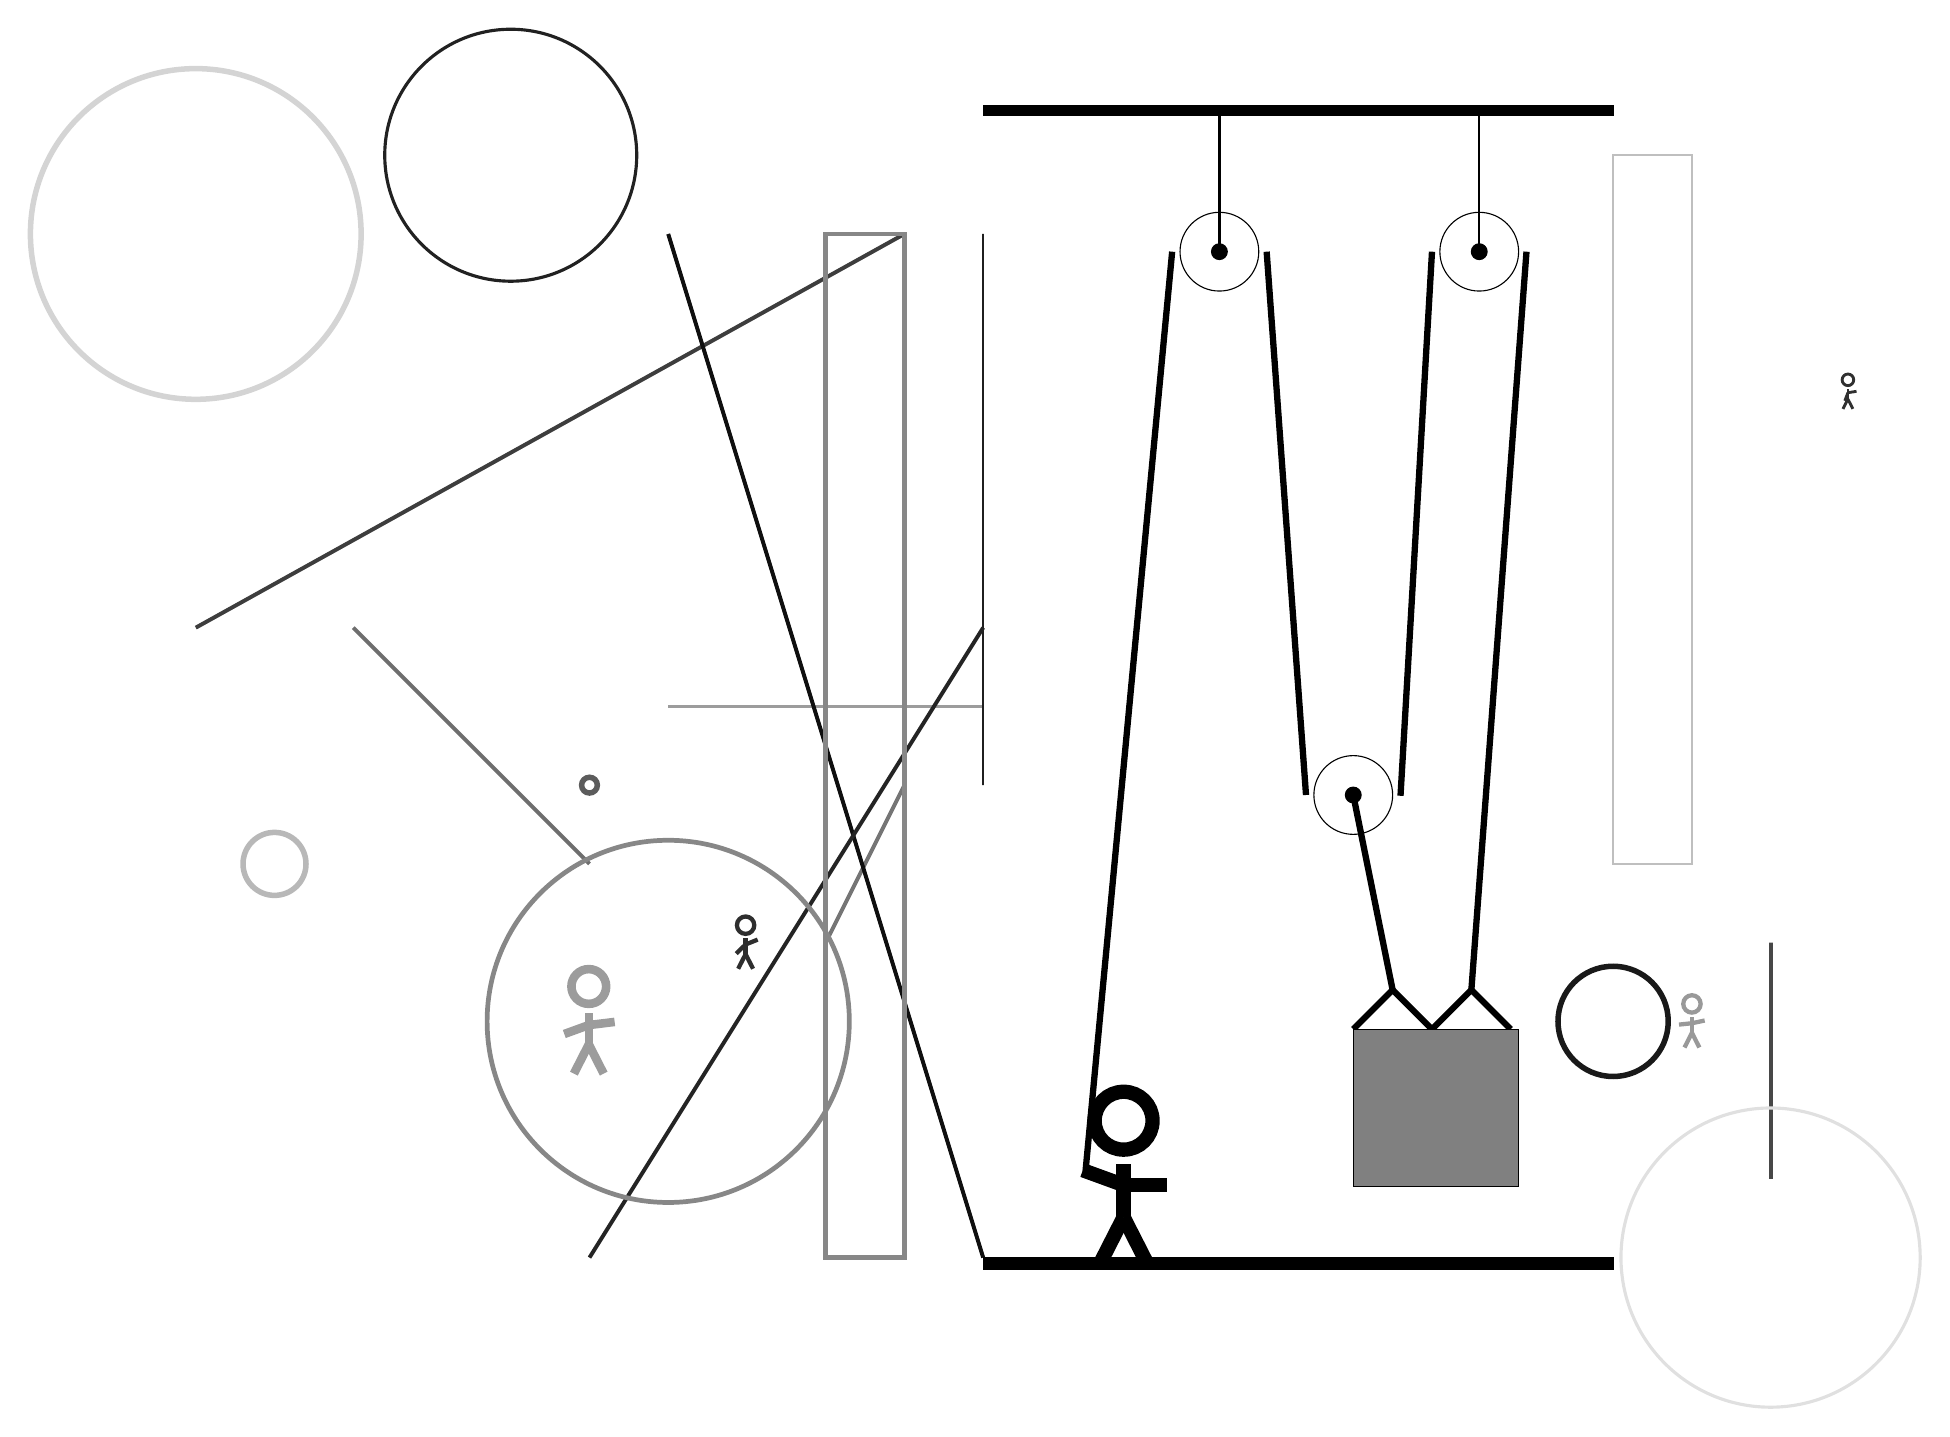
\begin{tikzpicture}
			%%%%% START %%%%%
			
			\draw[fill=black] (-2, 11.5) rectangle (6, 11.625);
			
			\draw (1, 9.775) circle (0.5);
			\draw[fill=black] (1, 9.775) circle (0.1);
			\draw[thick] (1, 9.775) -- (1, 11.5);
			
			\draw (4.3, 9.775) circle (0.5);
			\draw[fill=black] (4.3, 9.775) circle (0.1);
			\draw[thick] (4.3, 9.775) -- (4.3, 11.5);
			
			\draw (2.7, 2.875) circle (0.5);
			\draw[fill=black] (2.7, 2.875) circle (0.1);
			
			\draw[line width=0.8mm]  (2.7, -0.1) -- (3.2, 0.4) -- (3.7, -0.1) -- (4.2, 0.4) -- (4.7, -0.1);
			\draw[fill=black!50] (2.7, -0.1) rectangle (4.8, -2.1);
			
			\draw[line width=0.8mm](-0.7, -1.9) -- (0.4, 9.775);
			\centerarc[line width=0.8mm](1, 9.775)(0:180:0.6);
			\draw[line width=0.8mm](1.6, 9.775) -- (2.1, 2.875);
			\centerarc[line width=0.8mm](2.7, 2.875)(180:370:0.6);
			\draw[line width=0.8mm] (3.3, 2.865) -- (3.7, 9.775);
			\centerarc[line width=0.8mm](4.3, 9.775)(0:180:0.6);
			\draw[line width=0.8mm](4.2, 0.4) -- (4.9, 9.775);
			\draw[line width=0.8mm] (3.2, 0.4) -- (2.7, 2.875);
			
			\node at (-0.2, -2) {\Strichmaxerl[10][-20][0]};
			
			\draw[line width=0.5mm, color=black!57](-7, 2) -- (-10, 5);
			
			\draw[line width=0.5mm, color=black!76](-3, 10) -- (-12, 5);
			\draw[line width=0.5mm, color=black!54](-4, 1) -- (-3, 3);
			\node[line width=0.6mm, color=black!40] at (7, 0) {\Strichmaxerl[3][6][12]};
			\draw[line width=0.5mm, color=black!72] (8, 1) rectangle (8, -2);
			
			\draw[line width=0.3mm, color=black!39] (-2, 4) rectangle (-6, 4);
			\node[line width=0.5mm, color=black!81] at (9, 8) {\Strichmaxerl[2][69][9]};
			\draw[line width=0.2mm, color=black!25] (6, 2) rectangle (7, 11);
			\draw[line width=0.2mm, color=black!88] (-2, 10) rectangle (-2, 3);
			
			\node[line width=0.2mm, color=black!39] at (-7, 0) {\Strichmaxerl[6][20][7]};
			
			\draw [line width=0.7mm, color=black!90](6, 0) circle (0.7);
			\draw [line width=0.4mm, color=black!12](8, -3) circle (1.9);
			\draw [line width=0.7mm, color=black!28](-11, 2) circle (0.4);
			
			\draw[line width=0.5mm, color=black!94](-6, 10) -- (-2, -3);
			\draw [line width=0.7mm, color=black!17](-12, 10) circle (2.1);
			\node[line width=0.6mm, color=black!82] at (-5, 1) {\Strichmaxerl[3][44][22]};
			
			\draw[line width=0.5mm, color=black!86](-2, 5) -- (-7, -3);
			
			\draw [line width=0.7mm, color=black!64](-7, 3) circle (0.1);
			\draw [line width=0.4mm, color=black!87](-8, 11) circle (1.6);
			\draw [line width=0.6mm, color=black!47](-6, 0) circle (2.3);
			\draw[line width=0.6mm, color=black!47] (-4, -3) rectangle (-3, 10);
			
			
			\draw[fill=black] (-2, -3) rectangle (6, -3.15);
			
			%%%%% END %%%%%
		\end{tikzpicture}
	\end{figure}	
\end{document}